\chapter{Materials}\label{chap:materials}

%We have worked on two types of dataset. For, first data we have 2d images of fully developed zebrafish, showing complete anatomy. For, this data we have presented segmentation and quantification methodology. Second data consist of 3d temporal data of zebrafish vasculature. For, this we presented a technique for temporal vasculature growth. 

Zebrafish embryo images are collected at Center for Nuclear Receptors and Cell Signaling, Department of Biology and Biochemistry, University of Houston. Zebrafish (Danio rerio) are reared and maintained at $28.5^{\circ}$ C as previously described \cite{westerfield00}, and in accordance to the standard operating protocols approved by the Institutional Animal Care and Use Committee at University of Houston. A stable line of Tg(kdrl:EGFP)$mitfa^{b692}$ is generated by crossing Tg(kdrl:EGFP) with $mitfab^{692/b692}$ (Zebrafish International Resource Center, Eugene, OR) to facilitate GFP visualization without obstruction from melanophores. Embryos are collected from natural mating and staged accordingly \cite{Kimmel95}.

Two dimensional data is acquired for ISV and CVP analysis. Three dimensional time lapse data is acquired to study overall growth in vasculature of zebrafish. 

\section{Two Dimensional Data}
Zebrafish embryos are treated with chemicals selected from phase I of ToxCast chemical library (http://www.epa.gov/ncct/toxcast/chemicals.html) and solubilized in dimethyl sulfoxide (DMSO).

\subsection{Chemical Treatments}
Tg(kdrl:EGFP) $mitfa^{b692}$ embryos are harvested in a petri dish after mating. At approximately 3 hpf, embryos are sorted and placed in 6-well plates (n = 20), followed by a single chemical treatment without renewal at 100 nM, 250 nM, 500 nM, 1 $\mu$ M, 10 $\mu$ M and 20 $\mu$ M, unless otherwise noted. Working dilution stocks of all chemicals are made such that the final concentration of the vehicle DMSO is at 0.1\%. Each well contained a final volume of 3 mL of embryo medium, E3 (5 mM NaCl, 0.17 mM KCl, 0.33 mM CaCl2, 0.33 mM MgSO4). Control embryos are treated with 0.1\% DMSO. The embryos are incubated at $28.5^{\circ}$ C until 72 hpf, during which they are assessed for vascular perturbations. 

\subsection{Imaging}
At 72 hpf, control and treated embryos are manually dechorionated, if necessary, and anesthetized with 0.04\% MS-222 (Pentair Aquatic Eco-Systems, Apopka, FL). Embryos are manually oriented and imaged using a 4X objective on an Olympus IX51 fluorescence microscope equipped with an Olympus XM10 camera and cellSens Dimension software (Olympus, Center Valley, PA).

\begin{figure}[htb] 
 \begin{center}
    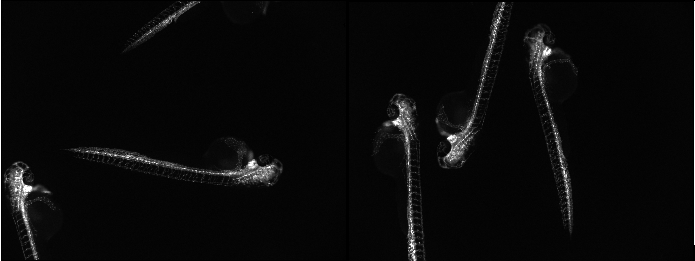
\includegraphics[scale=0.75]{figure/fishData.png}
  \end{center}
  \caption[Zebrafish full anatomy 2d dataset]{Original 2d images of zebrafish capturing zebrafish full anatomy.}
 \label{2dFish}
\end{figure}


\section{Three Dimensional Time - Lapse Data}

Zebrafish embryos are treated with Sodium (meta) arsenite (NaAsO$_{2}$) with 400 $\mu$g dosage. 

\subsection{Chemical Treatment}
Sodium (meta)arsenite (NaAsO$_{2}$) is purchased from Sigma-Aldrich (St. Louis, MO) and dissolved in ultra pure deionized water(vehicle). Tg(kdrl:EGFP)$mitfa^{b692}$ embryos are harvested in a petridish after mating. Then, they are sorted and placed in 6-wellplates (N = 10-30) in 3 mL of embryo medium, E3 (5 mM NaCl,0.17 mM KCl, 0.33 mM CaCl$_{2}$, 0.33 mM MgSo$^{4}$), followed by arsenite treatment at 400 $\mu$g/L (3.08 mM) without renewal. The embryos are incubated at $28.5^{\circ}$C until 72 hpf, at which they are manually dechorionated, if necessary, and assessed for vascular perturbation and other developmental malformations. For determining the window of effect, embryos are treated with arsenite at 400 $\mu$g/Lat 0-24 hpf, 24-48 hpf, or 48-72 hpf. After exposure time is complete, embryos are washed multiple times and allowed to continue to develop in E3 at $28.5^{\circ }$C until assessment at 72 hpf.For RT-qPCR, 30 embryos are pooled as one biological sample in 3 mL of E3 and treated with arsenite at 10 $\mu$g/L, 50 $\mu$g/L, 100 $\mu$g/L, 200 $\mu$g/L, or 400 $\mu$g/L up to 72 hpf. To examine RNA levels at different time points via RT-qPCR, embryos are treated with arsenite at 400 mg/L up to 18 hpf, 20 hpf, 24 hpf, 28 hpf, or 48 hpf. Control embryos are treated with vehicle.


\subsection{Imaging}

72 hpf control and arsenite-treated Tg(kdrl:EGFP)$mitfa^{b692}$ embryos are manually dechorionated, if necessary, and anesthetized with 0.04\% MS-222 (Pentair Aquatic Eco-systems, Apopka, FL). Embryos are then manually oriented and mounted in 0.8\%low-melt agarose (LMA; Sigma), and imaged using an Olympus Fluoview 1000 confocal fluorescence microscope with a 4X or 20X objective and 50 or 30 z-plane optical slices, respectively. Images are then rendered by Olympus Fluoview software and projection are generated using ImageJ. Brightfield images are captured with a Nikon DS-Fi1 color camera attached to a Nikon AZ100M microscope with a 4X objective and 25 z-plane optical slices, and then rendered by Nikon NIS-Elements software.2.7. 

\subsection{Time-lapse imaging}

Tg(kdrl:EGFP)$mitfa^{b692}$ embryos are treated with arsenite, as described above. At approximately 18 hpf, control and treatede mbryos are manually dechorionated, anesthetized with 0.04\%MS-222 and mounted in 0.3\% LMA on MatTek glass bottom dishes (MatTek Corporation, Ashland, MA). The 0.3\% LMA mounting media is supplemented with 0.04\% MS-222 and arsenite at concentrations matching to that of the exposure solutions. E3 with MS-222and arsenite is added following LMA solidification and the dishes are sealed with parafilm. 100 z-plane optical slices are acquiredon an Olympus Fluoview 1000 confocal fluorescence microscope over a span of 15 h with 15 min time intervals. Images are then processed by Olympus Fluoview software and projections are animated into a time-lapse movie using ImageJ.

\begin{figure}[htb] 
 \begin{center}
    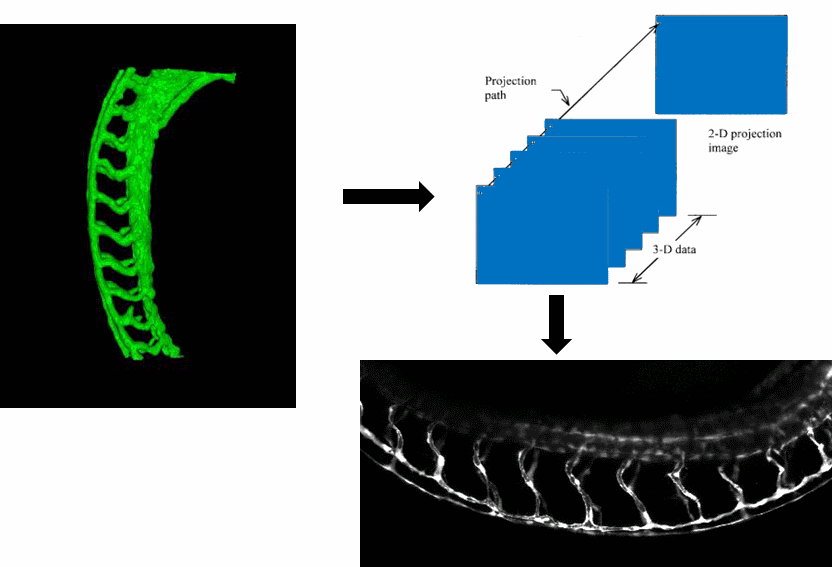
\includegraphics[scale=0.5]{figure/projection.png}
  \end{center}
  \caption[Maximum intensity projection]{Maximum intensity projection is computed by selecting the brightest voxel along z-axis.}
 \label{mip}
\end{figure}

\begin{figure}[htb] 
 \begin{center}
    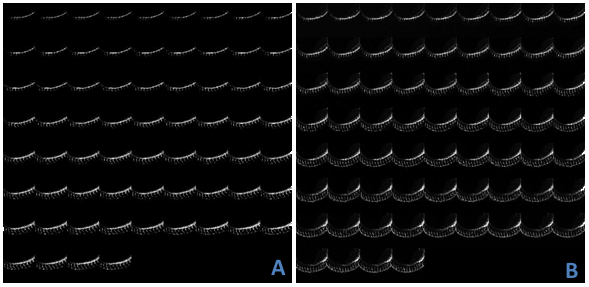
\includegraphics[scale=0.75]{figure/mon.png}
  \end{center}
  \caption[Zebrafish vasculature dataset]{(A) Vascular development for unexposed embryo. (B) Vascular development for arsenic exposed embryo.}
 \label{2dVascular}
\end{figure}

Images are generated in TIFF format with 8-bit intensity depth. Image size is 512 pixels by 512 pixels and 640 pixels by 480 pixels. Maximum Intensity projection (MIP) (fig. \ref{mip}) is computed for stack of images. MIP algorithm selects the brightest voxel along the z-axis and projects it on the orthogonal image plane. Figure \ref{2dVascular} shows MIPs for unexposed and exposed embryo.